%15 min preso!
\documentclass[xcolor=table,aspectratio=169]{beamer}
\usepackage{beamerthemesplit}
\usepackage{wrapfig}
\usetheme{SPbGU}
\usepackage{pdfpages}
\usepackage{amsmath}
\usepackage{cmap}
\usepackage[T2A]{fontenc}
\usepackage[utf8]{inputenc}
\usepackage[english]{babel}
\usepackage{indentfirst}
\usepackage{amsmath}
\usepackage{tikz}
\usepackage{multirow}
\usepackage[noend]{algpseudocode}
\usepackage{algorithm}
\usepackage{algorithmicx}
\usepackage{fancyvrb}
\usepackage{hyperref} 
\usetikzlibrary{calc}
\usetikzlibrary{shapes,arrows}
\usetikzlibrary{arrows,automata}
\usetikzlibrary{positioning}

\usepackage{tabularx}
\newcolumntype{Y}{>{\raggedleft\arraybackslash}X}

\renewcommand{\thealgorithm}{}

\newtheorem{mytheorem}{Theorem}
\renewcommand{\thealgorithm}{}

\newcommand{\tikzmark}[1]{\tikz[overlay,remember picture] \node (#1) {};}
\def\Put(#1,#2)#3{\leavevmode\makebox(0,0){\put(#1,#2){#3}}}

\newcommand{\ltz}{$< 1$}


\tikzset{
    state/.style={
           rectangle,
           rounded corners,
           draw=black, very thick,
           minimum height=2em,
           inner sep=2pt,
           text centered,
           },
}

\beamertemplatenavigationsymbolsempty

\title[Syntactic guided data analysis group]{PL\&T: Syntactic guided data analysis group}
\institute[PL\&T@SPbSU]{
Saint Petersburg State University
}

% То, что в квадратных скобках, отображается в левом нижнем углу.
\author[Semyon Grigorev]{Semyon Grigorev}

\date{March 22, 2022}

\begin{document}
{
\begin{frame}[fragile]
  \begin{table}
  \centering
  
\includegraphics[height=1.5cm]{pictures/SPbGU_Logo.png}
  %\begin{tabularx}{\linewidth}{XcX}
    %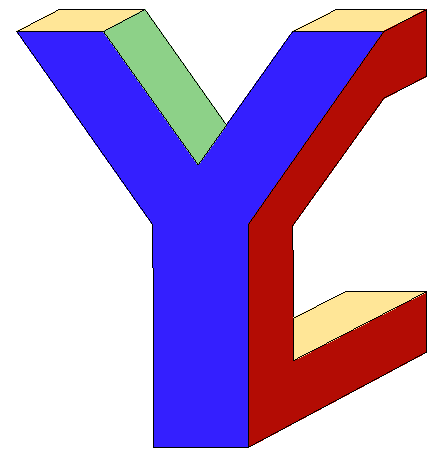
\includegraphics[height=1.5cm]{pictures/YC_logo.pdf} \hfill
    %& \begin{minipage}[t]{0.3\textwidth}\center \vspace{-1cm}  %Huawei-SPbSU Open Day 2021
    %  \end{minipage}
    %& \hfill 
\includegraphics[height=1.5cm]{pictures/SPbGU_Logo.png}
  %\end{tabularx}
  \end{table}
  \titlepage
\end{frame}
}

%for the presentation. muchbetter if more details of staff(name,education,skills,expertise,etc.) and research directions&results.


\begin{frame}[fragile]
  \frametitle{Group Info}  
  \begin{itemize}
      \item Established in 2012
      \item Lead: Semyon Grigorev
      \begin{itemize}
        \item PhD (2016), Associate professor (2016, SPbSU)
        \item dblp: \href{https://dblp.org/pid/181/9903.html}{https://dblp.org/pid/181/9903.html}
        \item h-index (scopus): 5
        \item \href{s.v.grigoriev@spbu.ru}{s.v.grigoriev@spbu.ru}
      \end{itemize}
      \item PhD students: 2
      \item Master's degree students: 5
      \item Bachelor's degree students: 6
      \item Publications
      \begin{itemize}
        \item Total: > 30
        \item Scopus: 25 
      \end{itemize}
      \item Research areas
      \begin{itemize}
        \item Formal languages constrained path querying
        \item High-performance graph analysis
        \item High-level languages for high-performance computing
      \end{itemize}
    \end{itemize}
\end{frame}

\begin{frame}[fragile]
  \frametitle{Formal Language Constrained Path Querying (FLPQ)}
  \begin{itemize}
    \item Formal languages as path constraints 
    \begin{itemize}
      \item Regular path querying (RPQ)
      \item Context-free path querying (CFPQ)
    \end{itemize} 
    \item Applications 
    \begin{itemize}
      \item Graph analysis
      \item Interprocedural static code analysis
      \item Graph database querying
    \end{itemize}
    \pause
    \item Research directions
    \begin{itemize}
      \item New algorithms development
      \item Complexity analysis
      \item New classes of languages investigation
      \item High performance algorithms implementation and evaluation 
    \end{itemize}
  \end{itemize}
\end{frame}

\begin{frame}[fragile]
  \frametitle{FLPQ: Team}
  \begin{itemize}
    \item Members 
    \begin{itemize}
      \item PhD students: Rustam Azimov, Ekaterina Shemetova
      \item Master students: Alexandra Istomina, Ilya Epelbaum
      \item Bachelor students: Valda Pogozelskaya, Timur Zinnatulin
    \end{itemize} 
    \item Skills 
    \begin{itemize}
      \item Formal language theory, parsing algorithms
      \item Graph theory, dynamic graph problems
      \item Algorithm design, data structures, algorithms complexity 
      \item Linear algebra, GraphBLAS
      \item RedisGraph, Neo4j, Cypher
    \end{itemize}
    \item Collaboration
    \begin{itemize}
      \item \href{https://team.inria.fr/links/}{INRIA LINKS}
      \item LDBC community
      \item RedisGraph team
      \item Neo4j team
    \end{itemize}
  \end{itemize}
\end{frame}

\begin{frame}[fragile]
  \frametitle{FLPQ: Results}
    \begin{itemize}
      \item Tools
      \begin{itemize}
        \item \href{https://github.com/JetBrains-Research/GLL4Graph}{GLL4Graph: CFPQ for Neo4j}
        \item \href{https://github.com/YaccConstructor/RedisGraph}{CFPQ for RedisGraph}
        \item \href{https://github.com/JetBrains-Research/CFPQ_PyAlgo}{CFPQ\_PyAlgo: set of GrpapBLAS-based FLPQ algorithms}
      \end{itemize}
      \item Papers (> 10)
      \begin{itemize}
        \item Multiple-Source Context-Free Path Querying in Terms of Linear Algebra (EDBT, Core A)
        \item Context-free path querying by matrix multiplication (GRADES-NDA@SIGMOD)
        \item Parser combinators for context-free path querying (Scala@ICFP)
      \end{itemize} 
    \end{itemize}
\end{frame}

\begin{frame}[fragile]
  \frametitle{High-Performance Graph Analysis}
  \begin{itemize}
    \item Linear algebra based algorithms for graph analysis
    \begin{itemize}
      \item Sparse linear algebra
      \item GraphBLAS
    \end{itemize} 
    \pause
    \item Research directions
    \begin{itemize}
      \item Portable multi-GPGPU implementation of GraphBALS-like API
      \item GraphBLAS-based algorithms design, implementation and evaluation
      \item GraphBLAS API analysis
    \end{itemize}
  \end{itemize}
\end{frame}

\begin{frame}[fragile]
  \frametitle{High-Performance Graph Analysis: Team}
  \begin{itemize}
    \item Members 
    \begin{itemize}
      \item Master students: Egor Orachev, Vladimir Kutuev
      \item Bachelor students: Gleb Marin
    \end{itemize} 
    \item Skills 
    \begin{itemize}
      \item Algorithm design, data structures, graph algorithms
      \item Linear algebra, sparse linear algebra, GraphBLAS
      \item C/C++, CUDA, OpenCL, OpenMP, GPGPU, Python 
    \end{itemize}
    \item Collaboration
    \begin{itemize}
      \item GraphBLAS community
      \item LDBC community
    \end{itemize}
  \end{itemize}
\end{frame}

\begin{frame}[fragile]
  \frametitle{High-Performance Graph Analysis: Results}
    \begin{itemize}
      \item Tools
      \begin{itemize}
        \item \href{https://github.com/JetBrains-Research/spla}{Spla: sparse linear algebra framework for multi-GPU computations based on OpenCL}
        \item \href{https://github.com/JetBrains-Research/spbla}{SPbLA: library of GPGPU-powered sparse boolean linear algebra operations}    
        \item \href{https://github.com/JetBrains-Research/ldbc_graphalytics}{LDBC Graphalytics extension for evaluation of formal language constrained path querying}    
      \end{itemize}
      \item Papers 
      \begin{itemize}
        \item SPbLA: The Library of GPGPU-Powered Sparse Boolean Linear Algebra Operations (GrAPL@IPDPS)
        \item Evaluation of the context-free path querying algorithm based on matrix multiplication (GRADES-NDA@SIGMOD)
      \end{itemize} 
    \end{itemize}
\end{frame}

\begin{frame}[fragile]
  \frametitle{High-Level Languages For High-Performance Computing (HLL for HPC)}
  In collaboration with Daniil Berezun
  \begin{itemize}    
  \item High-level languages for GPGPU programming and HLS
  \item \href{https://www.lift-project.org/}{LIFT}, AnyDSL, Futhark
  \pause
  \item Research directions
  \begin{itemize}
    \item Fusion-like optimization for sparse linear algebra routines (distillation)
    \item Sparse linear algebra in functional language: type safe, fusion-friendly, natural divide-and-conquer parallelism
    \item Special hardware for sparse linear algebra
  \end{itemize}
  \end{itemize}
\end{frame}

\begin{frame}[fragile]
  \frametitle{HLL for HPC: Team}
  \begin{itemize}
    \item Members 
    \begin{itemize}
      \item Daniil Berezun
      \item Master students: Alexey Turin
      \item Ekaterina Vinnik, Kirill Garbar, Artiom Chernikov
    \end{itemize} 
    \item Skills 
    \begin{itemize}
      \item Algorithm design, data structures
      \item Program optimization, program transformation
      \item Linear algebra, sparse linear algebra, GraphBLAS
      \item Functional programming (Haskell, F\#), OpenCL, GPGPU, FPGA 
    \end{itemize}
    \item Collaboration
    \begin{itemize}
      \item Geoff William Hamilton
    \end{itemize}
  \end{itemize}
\end{frame}

\begin{frame}[fragile]
  \frametitle{HLL for HPC: Results}
    \begin{itemize}
      \item Tools
      \begin{itemize}
        \item \href{https://github.com/YaccConstructor/Distiller}{Distiller: fusion-like optimization for sparse linear algebra routines}
        \item Contribution to \href{https://github.com/sedwards-lab/fhw}{FHW: functional program to hardware translator}    
        \item Contribution to \href{https://github.com/tommythorn/Reduceron}{Reduceron: specialized processor for functional programms}    
        \item \href{https://github.com/YaccConstructor/Brahma.FSharp}{Brahma.FSharp: F\# to OpenCL C translator and respective runtime}
      \end{itemize}
      \item Papers 
      \begin{itemize}
        \item Optimizing GPU programs by partial evaluation (PPoPP, Core A)
        \item Distilling Sparse Linear Algebra (SRC@ICFP)
      \end{itemize} 
    \end{itemize}
\end{frame}



\begin{frame}[fragile] \frametitle{Educational Activities}
  \begin{itemize}
  \item Research projects for students (bachelor, master, PhD)
  \item Lectures
  \begin{itemize}
  \item \href{https://github.com/JetBrains-Research/formal-lang-course}{Formal language theory and parsing algorithms}
  \item Algorithms and data structures
  \item Graph theory
  \item Introduction to machine learning
  \end{itemize}
\end{itemize}
\end{frame}

\end{document}
